\chapter{Etapas de Desenvolvimento e Implementação}
\label{ch::imp-test}

\section{Introdução}
\label{sec::imp-test:intro}

Para o sucesso deste projeto foi essencial delinear uma estratégia de investigação. Esta divide-se em 3 partes: reconstrução dos hologramas, compressão dos hologramas reconstruídos, e determinação das métricas de compressão. A cada uma destas fases atribuíram-se objetivos para a sua profícua execução:

\begin{enumerate}
    \item Reconstrução dos hologramas:
    \begin{enumerate}
        \item Estudar a holografia;
        \item Estudar as funções originais em MATLAB do Projecto JPEG Pleno;
        \item Transcrever estas funções para a linguagem de programação Python;
        \item Comparar o \textit{output} entre as funções originais em MATLAB e as respetivas transcrições em Python;
        \item Desenvolver um \textit{script} para reconstruir cada holograma em 16 vistas distintas.
    \end{enumerate}

    \item Compressão dos hologramas reconstruídos:
    \begin{enumerate}
        \item Estudar o uso do \ac{kdu};
        \item Automatizar a execução dos \textit{scripts} e \textit{softwares} envolvidos;
        \item Implementar um \textit{script} para compressão (com e sem transformada de cor em diferentes \textit{bitrates}) e descompressão dos hologramas reconstruídos.
    \end{enumerate}

    \item Determinação das métricas de compressão:
    \begin{enumerate}
        \item Calcular o débito com a métrica \ac{PSNR} entre os hologramas originais e as imagens comprimidas;
        \item Determinar o melhor método de armazenamento dos débitos calculados;
        \item Implementar o \textit{output} dos resultados no método selecionado;
        \item Gerar gráficos dos resultados.
    \end{enumerate}
\end{enumerate}

As Secções subsequentes expõem o trabalho desenvolvido neste sentido e a Figura \ref{fig:projeto} esquematiza o processo final.

\begin{figure}[!htbp]
    \centering
    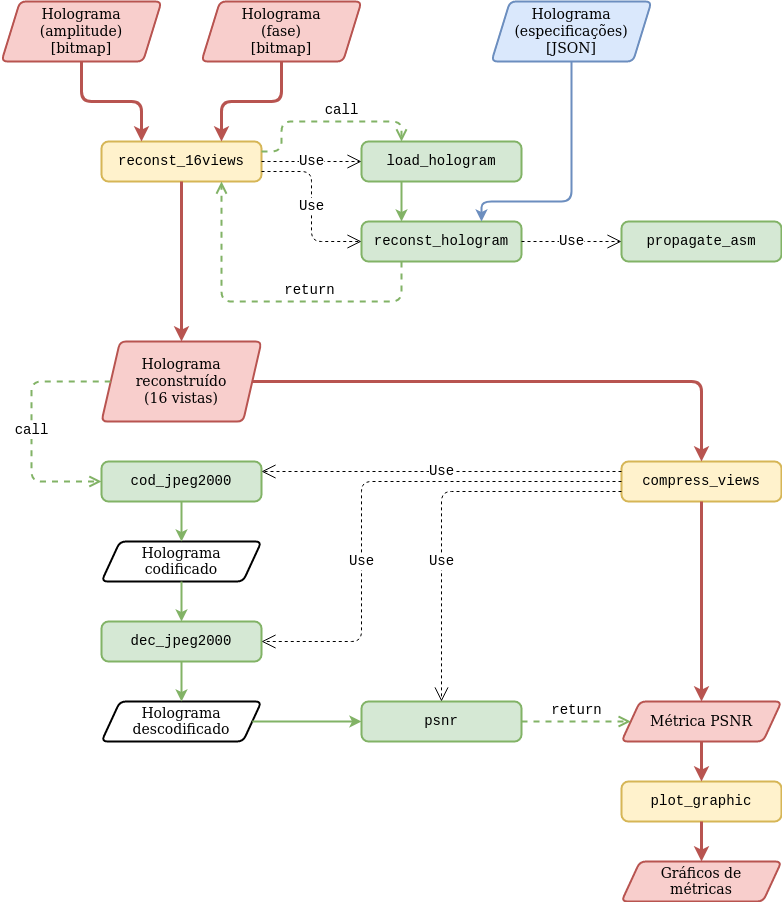
\includegraphics[width=\textwidth]{projeto}
    \caption
        [Diagrama do processo efetuado sobre um holograma para obtenção dos resultados.]
        {
            Diagrama do processo efetuado sobre um holograma para obtenção dos resultados.\\
            O caminho vermelho/amarelo representa o trajeto principal pelo qual o holograma sofre processamento. Os caminhos verdes detalham os processos intermédios correspondentes a um determinado processo do trajeto principal (a entrada é dada por ``\textit{call}'' e o retorno é dado por ``\textit{return}''). As dependências entre as principais funções são indicadas por ``\textit{Use}''.\\

        }
    \label{fig:projeto}
\end{figure}


\section{Reconstrução dos Hologramas}
\label{sec::imp-test:reconst-hologram}
% [X] Estudo holografia
% [X] estudo funções matlab
% [X] transcrever funções para scripts em python
% [X] comparar output entre funções de matlab e python para confirmar que os hologramas estão a ser reconstruídos corretamente
% [X] desenvolver script para reconstruir o mesmo holograma de 16 vistas diferentes

O projeto iniciou-se com uma pesquisa exaustiva sobre a ciência da holografia, a qual resultou no Estado da Arte resumido no Capítulo \ref{ch::estado-arte}.

Simultaneamente, foi efetuado um estudo das funções do \textit{software} desenvolvido no âmbito do projeto JPEG Pleno a fim de se poder fazer a respetiva transcrição para Python. O resultado deste estudo e transcrição encontra-se exposto nas tabelas \ref{tab:load_hologram}, \ref{tab:propagate_asm} e \ref{tab:reconst_hologram}.

% load hologram

\begin{table}[!htbp]
    \centering
    \caption{Resumo da documentação da função \texttt{load\_hologram}.}
    \label{tab:load_hologram}
    \begin{tabular}{p{1cm} p{10cm}}
        \hline
        \multicolumn{2}{l}{\bfseries Nome da função}\\
         & \verb|load_hologram|\\
        \hline
        \multicolumn{2}{l}{\bfseries Protótipo original em MATLAB}\\
         & \mintinline[breaklines]{matlab}{function [hologram] = load_hologram(ampli_path, phase_path)}\\
        \hline
        \multicolumn{2}{l}{\bfseries Protótipo transcrito em Python}\\
         & \mintinline{python}{def load_hologram(ampli_path, phase_path)} \\
        \hline\multicolumn{2}{l}{\bfseries Descrição}\\
         & Esta função carrega um holograma da base de dados b<>com a partir dos seus ficheiros de amplitude e fase.\\
        \hline\multicolumn{2}{l}{\bfseries \textit{Inputs}}\\
         & \verb|ampli_path|: Diretório do ficheiro da imagem da amplitude (caminho relativo ou absoluto).\\
         & \verb|phase_path|: Diretório do ficheiro da imagem da fase (caminho relativo ou absoluto).\\
        \hline\multicolumn{2}{l}{\bfseries \textit{Output}}\\
         & Modulação complexa do holograma (3 canais: \ac{RGB}).\\
        \hline\multicolumn{2}{l}{\bfseries Efeitos colaterais}\\
         & Não aplicável. \\
        \hline\multicolumn{2}{l}{\bfseries Dependências}\\
         & Não aplicável. \\
        \hline
    \end{tabular}
\end{table}


% propagate asm

\begin{table}[!htbp]
    \centering
    \caption{Resumo da documentação da função \texttt{propagate\_asm}.}
    \label{tab:propagate_asm}
    \begin{tabular}{p{1cm} p{10cm}}
        \hline
        \multicolumn{2}{l}{\bfseries Nome da função}\\
         & \verb|propagate_asm|\\
        \hline
        \multicolumn{2}{l}{\bfseries Protótipo original em MATLAB}\\
         & \mintinline[breaklines]{matlab}{function [v] = propagate_asm(u, pitch, wavelength, z)}\\
        \hline
        \multicolumn{2}{l}{\bfseries Protótipo transcrito em Python}\\
         & \mintinline[breaklines]{python}{def propagate_asm(u, pitch, wavelength, z)} \\
        \hline\multicolumn{2}{l}{\bfseries Descrição}\\
         & Esta função simula a propagação no plano complexo \verb|u| sobre a distância \verb|z| utilizando o \ac{ASM}.\\
        \hline\multicolumn{2}{l}{\bfseries \textit{Inputs}}\\
         & \verb|u|: Campo de onda de luz do plano de \textit{input} (um canal).\\
         & \verb|pitch|: Distância entre pixeis (em metros).\\
         & \verb|wavelength|: Comprimento de onda do canal de cor a propagar (em metros).\\
         & \verb|z|: Distância de propagação ao longo do eixo ótico (em metros).\\
        \hline\multicolumn{2}{l}{\bfseries \textit{Output}}\\
         & Campo de onda de luz no plano de destino (um canal).\\
        \hline\multicolumn{2}{l}{\bfseries Efeitos colaterais}\\
         & Não aplicável. \\
        \hline\multicolumn{2}{l}{\bfseries Dependências}\\
         & Não aplicável. \\
        \hline
    \end{tabular}
\end{table}


% reconst hologram

\begin{table}[!htbp]
    \centering
    \caption{Resumo da documentação da função \texttt{reconst\_hologram}.}
    \label{tab:reconst_hologram}
    \begin{tabular}{p{1cm} p{10cm}}
        \hline
        \multicolumn{2}{l}{\bfseries Nome da função}\\
         & \verb|reconst_hologram|\\
        \hline
        \multicolumn{2}{l}{\bfseries Protótipo original em MATLAB}\\
         & \mintinline[breaklines]{matlab}{function [recons] = reconsHologram(hologram, pitch, wavelengths, z, pupilPos, pupilSize)
         }\\
        \hline
        \multicolumn{2}{l}{\bfseries Protótipo transcrito em Python}\\
         & \mintinline[breaklines]{python}{def reconst_hologram(hologram, pitch, wavelengths, z, pupil_pos, pupil_size)} \\
        \hline\multicolumn{2}{l}{\bfseries Descrição}\\
         & Esta função reconstrói o holograma a uma distância \verb|z|, utilizando o \ac{ASM}. Permite o uso de uma janela para obter reconstruções de diferentes pontos de vista.\\
        \hline\multicolumn{2}{l}{\bfseries \textit{Inputs}}\\
         & \verb|hologram|: Holograma de modulação complexa (3 canais: \ac{RGB}). \\
         & \verb|pitch|: Distância entre pixeis (em metros).\\
         & \verb|wavelengths|: Comprimentos de onda de luz (em metros, 3 canais: \ac{RGB}).\\
         & \verb|z|: Distância de reconstrução (em metros).\\
         & \verb|pupilPos|: Posição da janela (em pixeis, canto superior direito).\\
         & \hspace{1cm} \textit{Valor por defeito.} \verb|[0, 0]|.\\
         & \verb|pupilSize|: Tamanho da janela (em pixeis, altura $\times$ largura).\\
         & \hspace{1cm} \textit{Valor por defeito.} \verb|None|.\\
        \hline\multicolumn{2}{l}{\bfseries \textit{Output}}\\
         & Reconstrução numérica do holograma (3 canais: \ac{RGB}).\\
        \hline\multicolumn{2}{l}{\bfseries Efeitos colaterais}\\
         & Não aplicável. \\
        \hline\multicolumn{2}{l}{\bfseries Dependências}\\
         & Função \verb|propagate_asm| (Tabela \ref{tab:propagate_asm}). \\
        \hline
    \end{tabular}
\end{table}


% reconstrução de holograma de 16 vistas

Estas funções foram compiladas num único \textit{script} Python. A fim de cumprir o \ref{obj:reconstruir_vistas}\textordmasculine~objetivo secundário, uma nova função, \verb|reconst_16views|, foi implementada (Tabela \ref{tab:reconst_16views}). Esta função está, portanto, encarregue de abrir um holograma, as respetivas especificações e reconstruí-lo em exatamente 16 vistas distintas. De notar que as especificações são fornecidas por um ficheiro JSON cujo conteúdo inclui:
\begin{itemize}
    \item \verb|holo_size|: Resolução do holograma (em pixeis);
    \item \verb|pitch|: Distância entre pixeis (em metros);
    \item \verb|wavelenghts|: Lista com os comprimentos de onda respetivos aos canais \ac{RGB} (em metros);
    \item \verb|z|: Distância de reconstrução (em metros);
    \item \verb|pupil_size|: Lista que contém o tamanho da janela de reconstrução (em pixeis).
\end{itemize}

\begin{table}[!htbp]
    \centering
    \caption{Resumo da documentação da função \texttt{reconst\_16views}.}
    \label{tab:reconst_16views}
    \begin{tabular}{p{1cm} p{10cm}}
        \hline
        \multicolumn{2}{l}{\bfseries Nome da função}\\
         & \verb|reconst_16views|\\
        \hline
        \multicolumn{2}{l}{\bfseries Protótipo em Python}\\
         & \mintinline[breaklines]{python}{def reconst_16views(hologram)} \\
        \hline\multicolumn{2}{l}{\bfseries Descrição}\\
         & Reconstrói o holograma fornecido por argumento em 16 vistas. \\
         & \textit{Processo.} Carrega o holograma (dois ficheiros \textit{bitmap}: amplitude e fase) e o respetivo ficheiro de especificações (formato JSON). Calcula as posições das 16 vistas tendo em conta o tamanho do holograma.\\
        \hline\multicolumn{2}{l}{\bfseries \textit{Inputs}}\\
         & \verb|hologram|: Nome do holograma a ser reconstruído.\\
         & \hspace{1cm} \textit{Valor por defeito.} ``\verb|dices4k|''.\\
        \hline\multicolumn{2}{l}{\bfseries \textit{Output}}\\
         & Não aplicável.\\
        \hline\multicolumn{2}{l}{\bfseries Efeitos colaterais}\\
         & Produz, dentro da pasta \verb|./reconst/|, uma nova pasta com o nome do holograma. O respetivo conteúdo incluirá as 16 vistas (ficheiros \verb|*.ppm|) correspondentes às reconstruções produzidas pela função.\\
        \hline\multicolumn{2}{l}{\bfseries Dependências}\\
         & Função \verb|load_hologram| (Tabela \ref{tab:load_hologram}); \\
         & Função \verb|reconst_hologram| (Tabela \ref{tab:reconst_hologram}). \\
         & \textit{Ver Figura \ref{fig:reconst_16views}.} \\
        \hline
    \end{tabular}
\end{table}

\begin{figure}[!htbp]
    \centering
    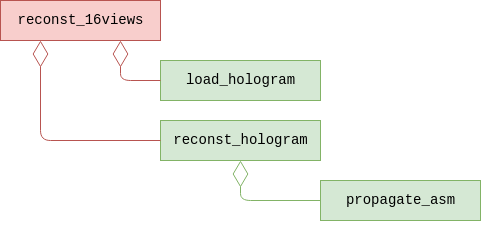
\includegraphics[scale=.6]{reconst_16views}
    \caption{Diagrama de dependências da função \texttt{reconst\_16views}.}
    \label{fig:reconst_16views}
\end{figure}

Todavia, havendo uma transcrição de funções entre linguagens de programação, exigiu-se uma forma de comprovar que as funções transcritas em Python são equivalentes às originais em MATLAB. Para este fim, delineou-se a seguinte estratégia:

\begin{enumerate}
    \item Etapa de implementação:
    \begin{enumerate}
        \item Transcrever as funções para Python (forme apresentado).
    \end{enumerate}
    
    \item Etapa de reconstrução:
    \begin{enumerate}
        \item Reconstruir os hologramas numa vista com as funções originais em MATLAB;
        \item Reconstruir os hologramas numa vista com as funções transcritas em Python.
    \end{enumerate}

    \item Etapa de comparação e resultados:
    \begin{enumerate}
        \item Comparar os hologramas produzidos pelos \textit{scripts} das duas linguagens através de uma análise visual a olho nu;
        \item Comparar os hologramas produzidos pelos \textit{scripts} das duas linguagens através da métrica \ac{PSNR}.
    \end{enumerate}
\end{enumerate}

Com o \textit{script} devidamente implementado e testado, prosseguiu-se com a seguinte fase do projeto relativo à compressão dos hologramas agora reconstruídos.


\section{Compressão dos Hologramas Reconstruídos}
\label{sec::imp-test:holo-compress}

TODO

% [x] estudar o uso de kdu
% [ ] automatização de execução dos softwares
% [ ] implementar script que comprime com e sem transformada de cor, e com bitrates: [0.1, 0.3, 0.6, 1.0, 1.5, 2.0, 2.5, 3.0, 3.5, 4.0, 4.5, 5.0], e descomprime as reconstruções do holograma





\subsection{Breve Estudo do \textit{Kakadu Software}}
\label{ssec::imp-test:holo-compress:estudo-kdu}

A fase de estudo do \ac{kdu} resultou no conhecimento exposto na Secção \ref{ssec::tecno-ferr:tecno-ferr:kdu}, onde se encontram descritos os dois comandos utilizados no âmbito do projeto.


\subsection{Implementação e Execução do \textit{Script} de Compressão}
\label{ssec::imp-tes:holo-compress:script}

TODO


\begin{table}[!htbp]
    \centering
    \caption{Resumo da documentação da função \texttt{compress\_views}.}
    \label{tab:compress_views}
    \begin{tabular}{p{1cm} p{10cm}}
        \hline
        \multicolumn{2}{l}{\bfseries Nome da função}\\
         & \verb|compress_views|\\
        \hline
        \multicolumn{2}{l}{\bfseries Protótipo em Python}\\
         & \mintinline[breaklines]{python}{def compress_views(hologram, ycbcr, rate)} \\
        \hline\multicolumn{2}{l}{\bfseries Descrição}\\
         & Comprimir os hologramas e calcular o \ac{PSNR}. \\
         & \textit{Processo.} Para cada vista, o holograma é codificado, descodificado e analisado em termos do \ac{PSNR}. São criados 16 ficheiros \verb|*.jp2| por pasta \verb|rate_n|, correspondentes às 16 vistas reconstruídas, assim como ficheiros JSON (um por holograma) na pasta \verb|kduOutput| com as métricas de compressão (\ac{PSNR}). \\
        \hline\multicolumn{2}{l}{\bfseries \textit{Inputs}}\\
         & \verb|hologram|: Nome do holograma a comprimir.\\
         & \hspace{1cm} \textit{Valor por defeito.} ``\verb|dices4k|''.\\
         & \verb|ycbcr|: \textit{Flag} que indica ao \ac{kdu} se deve ser efetuada uma transformada de cor.\\
         & \hspace{1cm} \textit{Valor por defeito.} \verb|False|.\\
         & \verb|rate|: número de \textit{bits} por amostra.\\
         & \hspace{1cm} \textit{Valor por defeito.} \verb|1.0|.\\
        \hline\multicolumn{2}{l}{\bfseries \textit{Output}}\\
         & Não aplicável.\\
        \hline\multicolumn{2}{l}{\bfseries Efeitos colaterais}\\
         & Armazena as imagens no formato \verb|*.jp2| nas pastas \verb|rate_n|, assim como os ficheiros JSON na pasta \verb|kduOutput|, segundo a seguinte árvore de diretórios:\\
         & \dirtree{%
            .1 ./.
            .2 kduOutput.
            .3 dices4k.
            .4 no\_ycbcr.
            .5 rate\_n\DTcomment{$n$: número de \textit{bits}}.
            .5 \ldots.
            .4 ycbcr.
            .3 diffuseCar4k\DTcomment{\textit{idem}}.
            .3 piano4k.
         } \\
        \hline\multicolumn{2}{l}{\bfseries Dependências}\\
        & Função \verb|cod_jpeg2000| (Tabela \ref{tab:cod_jpeg2000});\\
        & Função \verb|dec_jpeg2000| (Tabela \ref{tab:dec_jpeg2000});\\
        & Função \verb|psnr| (Tabela \ref{tab:psnr}).\\
        & \textit{Ver Figura \ref{fig:compress_views}.} \\
        \hline
    \end{tabular}
\end{table}



\begin{table}[!htbp]
    \centering
    \caption{Resumo da documentação da função \texttt{cod\_jpeg2000}.}
    \label{tab:cod_jpeg2000}
    \begin{tabular}{p{1cm} p{10cm}}
        \hline
        \multicolumn{2}{l}{\bfseries Nome da função}\\
         & \verb|cod_jpeg2000|\\
        \hline
        \multicolumn{2}{l}{\bfseries Protótipo em Python}\\
         & \mintinline[breaklines]{python}{def cod_jpeg2000(in_path, out_path, ycbcr, rate)} \\
        \hline\multicolumn{2}{l}{\bfseries Descrição}\\
         & Invoca ao sistema a execução do comando \verb|kdu_compress|, conforme descrito na Secção \ref{ssec::tecno-ferr:tecno-ferr:kdu}. \\
        \hline\multicolumn{2}{l}{\bfseries \textit{Inputs}}\\
         & \verb|in_path|: caminho do ficheiro de \textit{input}. \\
         & \verb|out_path|: caminho do ficheiro de \textit{output}. \\
         & \hspace{1cm} \textit{Valor por defeito.} ``\verb|out.jp2|''.\\
         & \verb|ycbcr|: \textit{flag} que indica ao \ac{kdu} se deve ser efetuada uma transformada de cor. \\
         & \hspace{1cm} \textit{Valor por defeito.} \verb|False|.\\
         & \verb|rate|: número de \textit{bits} por amostra. \\
         & \hspace{1cm} \textit{Valor por defeito.} \verb|1.0|.\\
        \hline\multicolumn{2}{l}{\bfseries \textit{Output}}\\
         & Não aplicável. \\
        \hline\multicolumn{2}{l}{\bfseries Efeitos colaterais}\\
         & Gera uma imagem no formato \verb|*.jp2| no diretório definido por \verb|out_path|. \\
        \hline\multicolumn{2}{l}{\bfseries Dependências}\\
         & Não aplicável. \\
        \hline
    \end{tabular}
\end{table}

\begin{table}[!htbp]
    \centering
    \caption{Resumo da documentação da função \texttt{dec\_jpeg2000}.}
    \label{tab:dec_jpeg2000}
    \begin{tabular}{p{1cm} p{10cm}}
        \hline
        \multicolumn{2}{l}{\bfseries Nome da função}\\
         & \verb|dec_jpeg2000|\\
        \hline
        \multicolumn{2}{l}{\bfseries Protótipo em Python}\\
         & \mintinline[breaklines]{python}{def dec_jpeg2000(in_path, out_path, ycbcr, rate)} \\
        \hline\multicolumn{2}{l}{\bfseries Descrição}\\
         & Invoca ao sistema a execução do comando \verb|kdu_expand|, conforme descrito na Secção \ref{ssec::tecno-ferr:tecno-ferr:kdu}. \\
        \hline\multicolumn{2}{l}{\bfseries \textit{Inputs}}\\
         & \verb|in_path|: caminho do ficheiro de \textit{input}. \\
         & \verb|out_path|: caminho do ficheiro de \textit{output}. \\
         & \hspace{1cm} \textit{Valor por defeito.} ``\verb|out.jp2|''.\\
         & \verb|ycbcr|: \textit{flag} que indica ao \ac{kdu} se deve ser efetuada uma transformada de cor. \\
         & \hspace{1cm} \textit{Valor por defeito.} \verb|False|.\\
         & \verb|rate|: número de \textit{bits} por amostra. \\
         & \hspace{1cm} \textit{Valor por defeito.} \verb|1.0|.\\
        \hline\multicolumn{2}{l}{\bfseries \textit{Output}}\\
         & Não aplicável. \\
        \hline\multicolumn{2}{l}{\bfseries Efeitos colaterais}\\
         & Gera uma imagem no formato \verb|*.tmp| no diretório definido por \verb|out_path|. \\
        \hline\multicolumn{2}{l}{\bfseries Dependências}\\
         & Não aplicável. \\
        \hline
    \end{tabular}
\end{table}

\begin{table}[!htbp]
    \centering
    \caption{Resumo da documentação da função \texttt{psnr}.}
    \label{tab:psnr}
    \begin{tabular}{p{1cm} p{10cm}}
        \hline
        \multicolumn{2}{l}{\bfseries Nome da função}\\
         & \verb|psnr|\\
        \hline
        \multicolumn{2}{l}{\bfseries Protótipo em Python}\\
         & \mintinline[breaklines]{python}{def psnr(p1, p2)} \\
        \hline\multicolumn{2}{l}{\bfseries Descrição}\\
         & Calcula a métrica de compressão \ac{PSNR} entre duas imagens. \\
        \hline\multicolumn{2}{l}{\bfseries \textit{Inputs}}\\
         & \verb|p1|: caminho para a primeira imagem. \\
         & \verb|p2|: caminho para a segunda imagem. \\
        \hline\multicolumn{2}{l}{\bfseries \textit{Output}}\\
         & Valor calculado do \ac{PSNR}. \\
        \hline\multicolumn{2}{l}{\bfseries Efeitos colaterais}\\
         & Não aplicável. \\
        \hline\multicolumn{2}{l}{\bfseries Dependências}\\
         & Não aplicável. \\
        \hline
    \end{tabular}
\end{table}


\begin{figure}[!htbp]
    \centering
    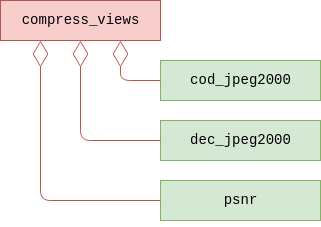
\includegraphics[scale=.6]{compress_views}
    \caption{Diagrama de dependências da função \texttt{compress\_views}.}
    \label{fig:compress_views}
\end{figure}



\subsection{Automatização dos \textit{Scripts}}
\label{ssec::imp-test:holo-compress:auto-script}

Para a otimização do processo de investigação neste projeto, foram criados dois \textit{scripts} adicionais, os quais trabalham em conjunto afim de automatizar todo este processo. São eles os seguintes:
\begin{enumerate}
    \item \textit{Makefile}: Introduz as 8 opções infra-apresentadas, as quais invocam o \textit{script} \verb|main.py|: 
        \begin{enumerate}
            \item \verb|reconst|: reconstrói o holograma fornecido por argumento em 16 vistas (Capítulo \ref{sec::imp-test:reconst-hologram} e Tabela \ref{tab:reconst_16views});
            \item \verb|compress|: executa o \textit{script} apresentado na Secção \ref{ssec::imp-tes:holo-compress:script};
            \item \verb|plot|: calcula os gráficos com os resultados de comparação da   compressão com e sem transformada de cor (Secção \ref{sec::imp-test:psnr});
            \item \verb|all|: executa os 3 itens anteriores;
            \item \verb|test|: opção utilizada na fase de \textit{debugging};
            \item \verb|install|: instala pacotes no sistema operativo essenciais à execução dos \textit{scripts};
            \item \verb|clean|: remove os diretórios relativos a: hologramas reconstruidos, \textit{output} do \ac{kdu}, ficheiros JSON dos resultados do \ac{PSNR}, e ficheiros de \textit{cache} do Python;
            \item \verb|clean-compressed|: remove os diretórios relativos a: \textit{output} do \ac{kdu}, ficheiros JSON dos resultados do \ac{PSNR}, e ficheiros de \textit{cache} do Python.
        \end{enumerate}
    \item \verb|main.py|: \textit{script} Python que executa as primeiras 5 opções supra-mencionadas conforme o argumento passado pelo \textit{Makefile}. Faz uso das funções \verb|reconst_16views| (Tabela \ref{tab:reconst_16views}) e \verb|compress_views| (Tabela \ref{tab:compress_views}).
\end{enumerate}


% [X] estudar o uso de kdu
% [X] automatização de execução dos softwares
% [ ] implementar script que comprime com e sem transformada de cor, e com bitrates: [0.1, 0.3, 0.6, 1.0, 1.5, 2.0, 2.5, 3.0, 3.5, 4.0, 4.5, 5.0], e descomprime as reconstruções do holograma



\section{Determinação das Métricas de Compressão}
\label{sec::imp-test:psnr}

TODO

% [ ] calcular o débito com a métrica PSNR entre o holograma original e a imagem comprimida
% [ ] estudar qual a melhor forma de guardar os débitos calculados
% [ ] implementar no script a escrita dos dados num ficheiro json
% [ ] a partir dos ficheiros json gerados, criar gráficos para apresentar os resultados com uso da biblioteca matplotlib.pyplot


\section{Conclusões}
\label{sec::imp-test:conclusao}

TODO
